\chapter{估算软件规模} % Introduction chapter suppressed from the table of contents


\hypertarget{ux4e3aux4ec0ux4e48ux8981ux4f30ux89c4ux6a21}{%
\subsection{为什么要估规模}\label{ux4e3aux4ec0ux4e48ux8981ux4f30ux89c4ux6a21}}

规模可以帮我们:

\begin{enumerate}
\tightlist
\item
  依据历史数据策划,例如估算工作量、工期
\item
  归一(Normalize)不同项目,作比较
\item
  知道现在水平
\end{enumerate}

依据历史数据策划 先把项目分成组件,参考以往类似的组件所花工作量,估算整个项目的总工作量。规模大小可简单看成是组件的数量。 (如果是新开发,以前从未做过同类开发,就只能靠个人经验直接估算工作量(或工期), 但是如果以前做过类似的工作,就可以参考以前的历史数据估算。) 
规模可以帮我们把不同项目归一。例如,验收测试缺陷数无法比较,但缺陷率 (
=缺陷数 / 规模) 便可以比较; 生产率(= 规模 / 所花总工时) 便可比。

有了归一后可比较的系数,个人/团队便更清楚当前的水平(质量/生产率),是否在上升或下降。

\hypertarget{ux4e3aux4ec0ux4e48ux4e0dux5e94ux7528ux4ee3ux7801ux884cux6570loc}{%
\subsection{为什么不应用代码行数(LOC)}\label{ux4e3aux4ec0ux4e48ux4e0dux5e94ux7528ux4ee3ux7801ux884cux6570loc}}

在1996年前, IBM 一直使用代码行数估算规模。
之前一直都使用近似机器语言的Assembly Lang.,
但为了提升效率,引入了高层语言 PL/S,发现 不能再用代码行数来估算规模
因PL/S 只需要更少代码行数 也能完成同样功能:

%Screenshotfrom20221220202712.png

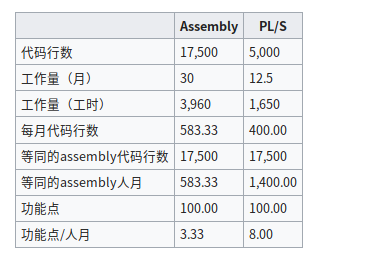
\includegraphics[width=10cm]{Screenshotfrom20221220202712.png}

上表是IBM(1968 - 1975)对两种编译器的统计:\\
每个月 PL/S产出代码行数(400) 反比 Assembly(583) 少

但是如果用功能点数便能真正反映生产率的提升: PL/S : 8.00 对比 Assembly
:3.33

\hypertarget{ux53eaux9002ux7528ux4e8eux7f16ux7801}{%
\subsubsection{只适用于编码}\label{ux53eaux9002ux7528ux4e8eux7f16ux7801}}

看下表,代码行数只能反应编程的工作量,但编码仅占项目总工作量的一部分
如果把项目按工作量分成以下五个部分 代码行数只能用于第二部分编码 (25\%)
其他4部分(30\% + 20\% + 15\% + 10\%)都不合适。

%Screenshotfrom20221220202832.png

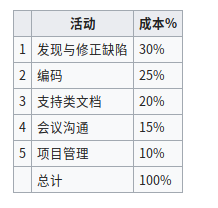
\includegraphics[width=10cm]{Screenshotfrom20221220202832.png}

\hypertarget{ux4e0eux529fux80fdux70b9ux6bd4ux8f83}{%
\subsubsection{与功能点比较}\label{ux4e0eux529fux80fdux70b9ux6bd4ux8f83}}

能估算好项目规模应可帮助我们更好估算工作量,规模应具备以下条件:

\begin{enumerate}
\tightlist
\item
  要和工作量有密切相关 - 应该与工作量强相关
\item
  要容易数得出来
\item
  容易在项目早期可以估算到
\end{enumerate}

功能点比较符合以上条件;只要功能需求明确,就可以估算出对应的功能点数。

只要需求明确便可以准确客观的估算功能点数。
因功能点估算已经是国际标准,基于功能点的度量数据可以与其他国家的标杆对比。

\hypertarget{ux600eux6837ux4f30sifp}{%
\subsection{怎样估SiFP}\label{ux600eux6837ux4f30sifp}}

有了功能性需求,并识别出系统范围,就可以开始估算功能点。:

\begin{enumerate}
\tightlist
\item
  数据功能(简称`实体')的数量 * 7 (实体是系统要管理的数据,)
\item
  业务功能(简称`行为')的数量 * 4.6 (行为可以简单看成是增删改查等功能)
\end{enumerate}

\begin{description}
\tightlist
\item[]
简化功能点数 = 上面 1 和 2 的总数
\end{description}

例如,附件例子一:潜水学校新开发项目:

\begin{itemize}
\tightlist
\item
  识别出3个实体和24个行为,得出简化功能点数131.4 = 3 * 7 + 24 * 4.6
\end{itemize}

潜水学校二次开发项目:
有些功能删除,有些功能变更,就需要分开计算动态功能点和静态功能点:

\begin{itemize}
\tightlist
\item
  静态功能点可以看成是整个系统的功能点数,所以变更的功能点数不会引起影响,但删除的话就需要减去。
\item
  动态功能点主要是用于估算本期开发项目的工作量,因为无论变更功能或者删除功能,都会导致有开发工作量,所以不能是零或负数。国际功能点的规定很简单,都加起来。
\end{itemize}

所以这次二次开发的动态功能点是:

\begin{description}
\item[]
\begin{description}
\tightlist
\item[]
2 * 7 + 11 * 4.6 (增加 两个实体和十一个行为)
\end{description}

+ 1 * 7 + 3 * 4.6 (变更 一个实体和三个行为)

+ 0 * 7 + 2 * 4.6 (删除 两个行为)

= 64.6 + 20.8 + 9.2
\end{description}

再加上 4.6 (因为有数据转换,所以需要加一个CFP,等于4.6)\\
最终动态功能点是99.2 (= 64.6 + 20.8 + 9.2 + 4.6)

静态功能点: 新开发 , 加上新增, 减去删除的功能点

\begin{description}
\item[]
\begin{description}
\tightlist
\item[]
= 131.4 + 64.6 - 9.2

= 186.6
\end{description}
\end{description}

\hypertarget{ux4eceux6545ux4e8bux70b9ux8f6cux7b80ux5316ux529fux80fdux70b9}{%
\subsection{从故事点转简化功能点}\label{ux4eceux6545ux4e8bux70b9ux8f6cux7b80ux5316ux529fux80fdux70b9}}

因故事点只是每个团队自己定义,无法用来作为组织级标准衡量规模,所以很多公司(尤其是银行)转用功能点来衡量软件开发规模。它不仅可用于公司内,也适用于行业标杆,功能点也适用于公司内或公司间结算,例如软件维护期里开发工作量变化很大,也难以事前预估,所以有些银行会按最终开发出来的功能点数结算使用部门付开发部的费用,减少争议。

虽然功能点分析源自70年代,但由于计算较复杂,一直未普及,有些人觉得IFPUG
FPA太复杂。针对这问题,国际功能点协会简化本来的功能点算法,推出简化功能点(SiFP),减少了估算的工作量与学习难度(例如,培训可以从以往的2天半降到半天)。因简化功能点不考虑实体/行为的复杂度,它与本来功能点的估算有\(\pm\)
15 \textasciitilde{} 20\% 偏差(详见附件例子)。
因敏捷团队是按每轮迭代估算(而不是一次性估整个项目),偏差就可以接受
(例如,2周一个迭代,偏差大概1.5天),所以SiFP
能适用于敏捷多次迭代估算。所以越来越多团队开始从故事点转简化功能点,但由于不熟识功能点估算是从用户角度估算,而非从开发工程师的视角看,团队初次估算SiFP通常有误。下面是某成都团队从故事点转简化功能点的案例:

\framebox{%
\begin{minipage}[t]{0.97\columnwidth}\raggedright
客户:我们以前一直使用故事点,为了更好做量化管理,我们新的项目开始使用简化功能点
- SiFP\\
我:好的,看一下你的估算表 。 。 。 。
为什么这两个功能要分成两个行为?\\
客户:这两个功能都挺复杂,估计需要很多开发工作量;我们以前用故事点估算时,也会分成两个故事点。\\
我:请注意,在功能点估算, 是否是一个行为,取决于它算不算是一个基本过程
如果俩行为互相依赖,不能单独作为基本过程,就不应该分开为2个功能点。很多团队刚开始用功能点,与你们一样,没有弄清楚基本过程的概念,还是从工程师的角度,估计开发时间的工作量来判断是一个功能还是两个功能?在故事点用这种方式估算习惯,但因为功能点是要同一个功能上需求,不能有功能点数的差异,所以不能用估计开发难易程度来判断。\\
客户:可否举个实例?\\
我:以网约车为例,是否可以分成以下9个''行为``?

%\href{文件:sifp_p50图.jpg}{600px}

\includegraphics[width=10cm]{sifpp50图.jpg}

\begin{enumerate}
\tightlist
\item
  预约申请
\item
  接收预约
\item
  检查是否有可用的车/司机
\item
  寻找其他可选
\item
  提供预约信息
\item
  处理预约
\item
  分派司机
\item
  接乘客
\item
  完成预约请求
\end{enumerate}

客户:是的,每个行为都要花一定开发工作量。\\
我:其实按SiFP只有4个行为,因头5个,和最后2个都要合并才可以成行为(详见附件)。
如果要能独立成行为,必须符合基本过程条件。
基本过程不是随便定的,它有规则,比如从网约车案例我们可以看到,``预约申请''本身不能算一个基本过程,虽然预约申请可能要很复杂的开发工作,但是因为它不能独立存在,必须依赖其它的行为才算完整。\\
例如,某公司财务系统有打印支票功能(用来付供应商),你觉得打印支票本身是否算基本过程?\\
客户:听完你网约车例子,应该不算;因打印支票只是付款流程的一个可选部分。\\
我:正确、算实体也应使用同样概念。例如,某人事管理系统,除了管理职工信息外,还有员工家属信息,因家属信息必须关连到员工信息,不能独立存在,所以家属信息本身不算是一个实体。你是否觉得你这表里的某些实体应合并?\\
客户:听完你的解释,同意我们这次计算有些实体应合并。\\
我:你们的功能点估算表没有明确区分新的迭代怎么处理变更与删除。
也没有明确动态功能点与静态功能点。\\
客户:我们表中有计算每次迭代的总功能点数。\\
我:你们可能有算每迭代的功能点,但难以看清后面迭代对应之前的变化。动态功能点是用来估算本本迭代的工作量,而静态功能点就是迭代后产品的功能点数。而且应该用表格形式把变更和删除累加在原本上一轮的功能上面,才可以更好看到迭代与迭代之间,功能上的变化。\\
所以不要误以为可以像之前故事点估算,按个人理解写上各种不同复杂程度的故事点例子便可。国际功能点手册里包含很多计算实例,来解释功能点计算,才能确保对同一套需求,每个人,依据用户需求,都能估算出同样的功能点数。我刚刚的例子全都可以从国际功能点手册里找到,你们不需要再发明车轮(reinvent
the wheel)。学功能点估算与写程序类似,必须多动手试。

建议你们读完网约车识别基本过程例子后,再读潜水学校两实例:

\begin{enumerate}
\tightlist
\item
  首次开发
\item
  增强功能与维护 (Enhancement)
\end{enumerate}

觉得已经把握好功能点计算原理,可尝试练习3+4,同样是首次开发+
增强功能与维护。\strut
\end{minipage}}

\hypertarget{ux603bux7ed3}{%
\subsubsection{总结}\label{ux603bux7ed3}}

虽然简化功能点(SiFP)比传统国际功能点IFPUG简单,容易学,但开发人员容易还是用工程师的视角来估算(本应用用户的视角),导致计算错误。所以要多看案例,并做练习才能把握(能参加培训会更好)。

\hypertarget{ux9644ux4ef6}{%
\section{附件}\label{ux9644ux4ef6}}

\hypertarget{ux7b80ux5316ux529fux80fdux70b9sifp-ux7b80ux4ecb}{%
\subsection{简化功能点(SiFP)
简介}\label{ux7b80ux5316ux529fux80fdux70b9sifp-ux7b80ux4ecb}}

 \textbf{它是做什么的?} \\
应用软件开发的客户需求可分成三类:

\begin{enumerate}
\tightlist
\item
  功能性需求
\item
  技术需求
\item
  质量需求
\end{enumerate}

第二类和第三类归为非功能性需求。功能点主要是针对功能性需求,目的是提供对客户有意义的功能点数,来客观地衡量软件规模。

 \textbf{该如何去做?} \\
简化功能点(SiFP)主要两类度量:

\begin{enumerate}
\tightlist
\item
  数据功能 - 实体 (逻辑文件 Logical File)
\item
  事务功能 - 行为(基本过程 Elementary Process)
\end{enumerate}

%\href{文件:功能点计数过程.jpg}{500px}

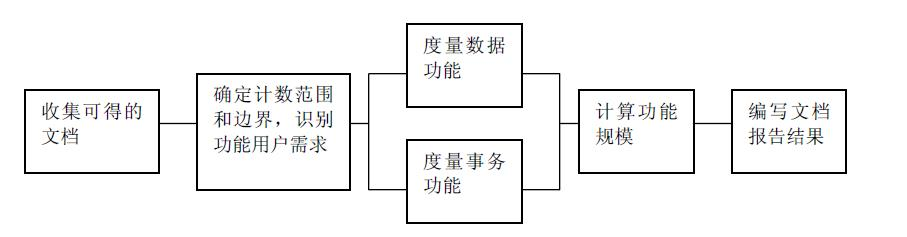
\includegraphics[width=10cm]{功能点计数过程.jpg}

\hypertarget{ux7b80ux5316ux529fux80fdux70b9ux4f30ux7b97ux6b65ux9aa4}{%
\subsubsection{简化功能点估算步骤:}\label{ux7b80ux5316ux529fux80fdux70b9ux4f30ux7b97ux6b65ux9aa4}}

\begin{enumerate}
\tightlist
\item
  确定功能点分析类型
\item
  识别分析范围和应用边界
\item
  计算数据类型功能点(Data Function)
\item
  计算交易类型功能点(Transaction Function)
\item
  计算功能点
\end{enumerate}

\hypertarget{ux4e09ux79cdsifpux8ba1ux7b97ux7c7bux578b}{%
\subsubsection{1:三种SiFP计算类型}\label{ux4e09ux79cdsifpux8ba1ux7b97ux7c7bux578b}}

\begin{itemize}
\tightlist
\item
  开发(Development )
\end{itemize}

\begin{description}
\item[]
\begin{description}
\tightlist
\item[]
DSFP = ADD + CFP
\end{description}
\end{description}

\begin{itemize}
\tightlist
\item
  应用 (Application or Baseline after the initial development)
\end{itemize}

\begin{description}
\item[]
\begin{description}
\tightlist
\item[]
ASFP = ADD
\end{description}
\end{description}

\begin{itemize}
\tightlist
\item
  更新/增强功能与维护 (Enhancement)
\end{itemize}

\begin{description}
\item[]
\begin{description}
\tightlist
\item[]
ESFP = ADD + CHG + DEL + CFP
\end{description}
\end{description}

%Screenshotfrom20221220202712.png

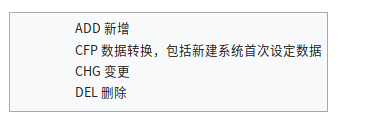
\includegraphics[width=10cm]{Screenshotfrom2022122020-31-37.png}

\hypertarget{ux8bc6ux522bux5206ux6790ux8303ux56f4ux548cux5e94ux7528ux8fb9ux754c}{%
\subsubsection{2:识别分析范围和应用边界}\label{ux8bc6ux522bux5206ux6790ux8303ux56f4ux548cux5e94ux7528ux8fb9ux754c}}

例子:用虚线标示系统边界:\\
%\href{文件:功能点计数P62_2.0.jpg}{500px}\\

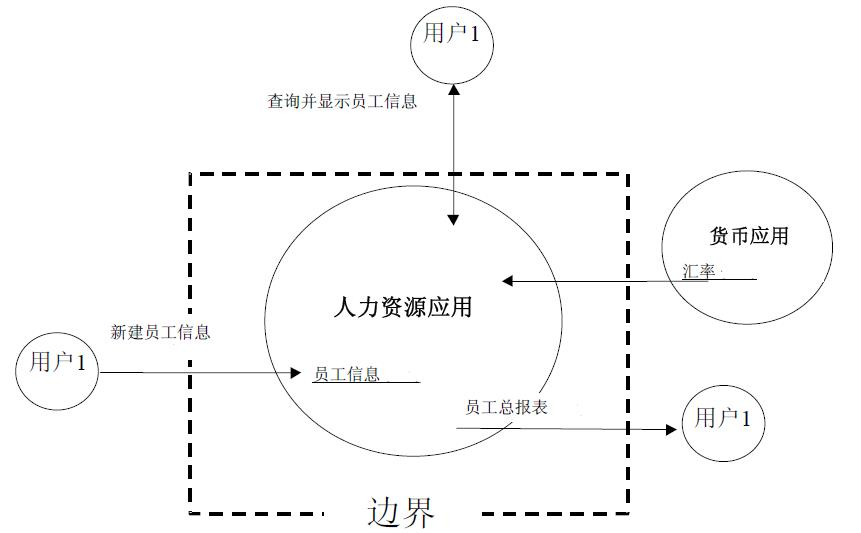
\includegraphics[width=10cm]{功能点计数P6220.jpg}

\hypertarget{ux8ba1ux7b97ux903bux8f91ux6587ux4ef6ux6570}{%
\subsubsection{3:计算逻辑文件数}\label{ux8ba1ux7b97ux903bux8f91ux6587ux4ef6ux6570}}

\begin{itemize}
\tightlist
\item
  关于计算规则,详见"逻辑文件"
\end{itemize}

\hypertarget{ux8ba1ux7b97ux57faux672cux8fc7ux7a0bux6570}{%
\subsubsection{4:计算基本过程数}\label{ux8ba1ux7b97ux57faux672cux8fc7ux7a0bux6570}}

\begin{itemize}
\tightlist
\item
  关于计算规则,详见"基本过程"
\end{itemize}

\hypertarget{ux8ba1ux7b97ux529fux80fdux70b9}{%
\subsubsection{5:计算功能点}\label{ux8ba1ux7b97ux529fux80fdux70b9}}

\begin{itemize}
\tightlist
\item
  每个逻辑文件 = 7.0 简化功能点
\item
  每个基本过程 = 4.6 简化功能点
\end{itemize}

\hypertarget{ux903bux8f91ux6587ux4ef6-logical-file}{%
\subsection{逻辑文件 Logical
File}\label{ux903bux8f91ux6587ux4ef6-logical-file}}

\textbf{(下面在计算实例里简称``实体'',方便理解)}

\begin{itemize}
\tightlist
\item
  用来储存内部或外部数据,是用户可识别的逻辑相关的数据组或控制信息组,在被度量应用边界内部维护。
\end{itemize}

\begin{description}
\tightlist
\item[]
(\textbf{用户可识别} -
指数据或事务需求是被用户和软件开发人员双方共同认同并理解的。
例如:用户和软件开发人员双方都认同人力资源应用有维护和存储员工信息的功能。)
\end{description}

\hypertarget{ux6ce8ux610f}{%
\paragraph{注意}\label{ux6ce8ux610f}}

逻辑文件包括两类不同的用户需求数据:

\begin{enumerate}
\tightlist
\item
  功能性数据
\item
  非功能性数据
\end{enumerate}

功能性数据是用来满足用户功能需求的数据。例如,销售、银行账号、供应商、人员等信息。\\
非功能数据主要是为了满足易用性(支撑下拉菜单所需的数据,可输入数据的上下范围等);或性能方面(用于查询数据的索引index);或可维护性(配置参数)。\\
只有第一类功能性数据才算是逻辑文件。\\

\hypertarget{ux57faux672cux8fc7ux7a0b-elementary-process}{%
\subsection{基本过程 Elementary
Process}\label{ux57faux672cux8fc7ux7a0b-elementary-process}}

基本过程是对用户有意义的最小活动单元。例如:添加员工的用户需求包括建立工资和家属信息。只有添加所有员工信息,才能创建员工信息记录。单独添加一些信息使添加员工业务处于不持续状态,只有员工工资和家属信息都添加后,这个活动单元才能完成且业务处于稳定状态。

\hypertarget{ux8bc6ux522bux57faux672cux8fc7ux7a0b}{%
\subsubsection{识别基本过程}\label{ux8bc6ux522bux57faux672cux8fc7ux7a0b}}

为了识别基本过程,需要执行以下活动:

\begin{itemize}
\tightlist
\item
  把功能用户需求分解为最小活动单元,使其满足下面条件:

  \begin{itemize}
  \tightlist
  \item
    对用户有意义\\
    例如:功能用户需求要求在应用中添加新员工的能力。\\
  \item
    构成一个完整的事务\\
    例如:用户定义的员工信息包括工资和家属信息。如果家属人数大于零,添加员工信息时必须包括家属信息。本例中,添加员工信息(不包括添加地址、工资和家属信息)不满足本规则。\\
  \item
    自包含\\
    例如:除非输入所有的必需信息并且完成所有处理步骤,如验证、计算、更新ILFs,添加过程才是自包含的。\\
  \item
    让应用程序的业务保持持续状态\\
    例如:添加员工的用户需求包括建立工资和家属信息。只有添加所有员工信息,才能创建员工信息记录。单独添加一些信息使添加员工业务处于不持续状态,只有员工工资和家属信息都添加后,这个活动单元才能完成且业务处于持续状态。\\
  \end{itemize}
\end{itemize}

识别活动单元为基本过程需要满足以上所有规则。\\

\hypertarget{ux8bc6ux522bux57faux672cux8fc7ux7a0bux4e3bux8981ux76eeux7684}{%
\subsubsection{识别基本过程主要目的}\label{ux8bc6ux522bux57faux672cux8fc7ux7a0bux4e3bux8981ux76eeux7684}}

基本过程的主要目的可识别为下列情形的一种:

\begin{itemize}
\tightlist
\item
  改变应用行为
\item
  维护一个或多个ILFs
\item
  呈现信息给用户
\end{itemize}

\hypertarget{ux5b9eux4f8bux8bc6ux522bux57faux672cux8fc7ux7a0b-ep-elementary-process}{%
\subsection{实例:识别基本过程 (EP elementary
process)}\label{ux5b9eux4f8bux8bc6ux522bux57faux672cux8fc7ux7a0b-ep-elementary-process}}

下面是某预约网约车过程:

%Screenshotfrom20221220203338.png

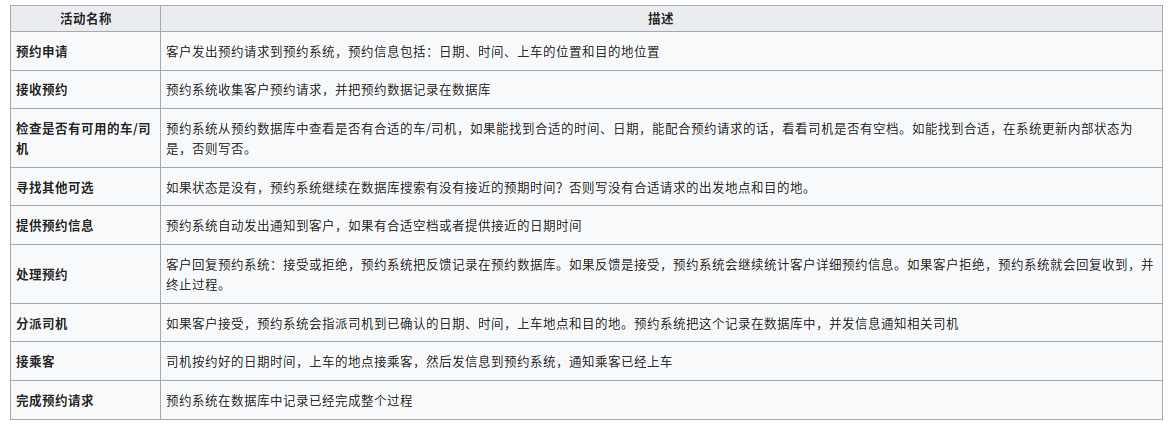
\includegraphics[width=10cm]{Screenshotfrom20221220203338.png}

\textbf{分析能否满足所有 EP 识别规则,判断能否独立成为基本过程 (EP
elementary process),部分例子}

\hypertarget{ux9884ux7ea6ux7533ux8bf7}{%
\subsubsection{预约申请}\label{ux9884ux7ea6ux7533ux8bf7}}

\begin{enumerate}
\tightlist
\item
  是否对用户有意义,客户功能需求的一部分?\textbf{是}
\item
  是否构成一个完整的事务?\textbf{否}:预约申请本身不是一个完整的交易,因为过程必须也包括预约请求信息,收到其它可选的档期这些步骤,都不可以分离。
\item
  是否自包含,可以独立存在?\textbf{否}:例如,接受预约申请;查看是否有档期,查看有没有其它接近的档期等,都是一些必须的相关步骤去完成这个基本过程。
\item
  是否让应用程序达到稳定状态?\textbf{否}:整个业务需求只能在收到预约信息,发送、接受、处理、反馈给客户才算是完成稳定状态。
\end{enumerate}

\hypertarget{ux5206ux6d3eux53f8ux673a}{%
\subsubsection{分派司机}\label{ux5206ux6d3eux53f8ux673a}}

\begin{enumerate}
\tightlist
\item
  是否对用户有意义,客户功能需求的一部分?\textbf{是}
\item
  是否构成一个完整的事务?\textbf{是}:分配到司机是一个完整的交易,包括收到司机的确认,把信息记录在系统中并通知司机。
\item
  是否自包含,可以独立存在?\textbf{是}:分配到司机本身可以独立存在。
\item
  是否让应用程序达到稳定状态?\textbf{是}:因为当司机被分配后,是完全满足业务的需要。
\end{enumerate}

\hypertarget{ux63a5ux4e58ux5ba2}{%
\subsubsection{接乘客}\label{ux63a5ux4e58ux5ba2}}

\begin{enumerate}
\tightlist
\item
  是否是客户功能需求?\textbf{是}
\item
  交易是否完整?\textbf{否}:接乘客本身不算一个完整的交易,因为预约系统必须也记录这个信息。
\item
  是否自包含,可以独立存在?\textbf{否}:确认预约申请是下面一个必须执行的过程,来完成这个基本过程。
\item
  是否让应用程序达到稳定状态?\textbf{否}:整个业务需求只能在和预约系统确认沟通,已经接到乘客,然后系统也把记录更新到预约系统才算完成。
\end{enumerate}

%Screenshotfrom2022122020-34-37.png

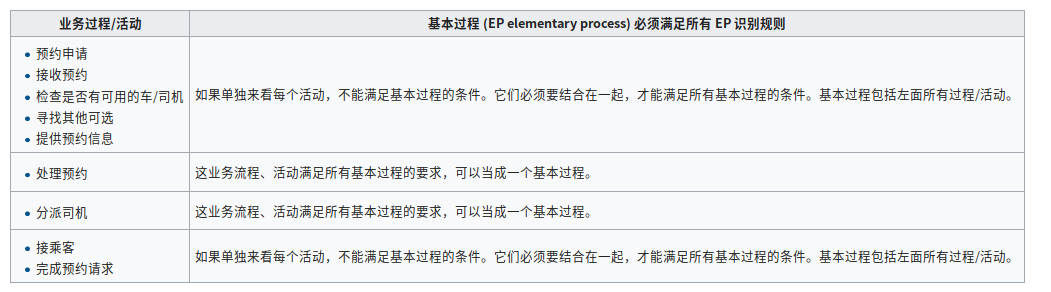
\includegraphics[width=10cm]{Screenshotfrom2022122020-34-37.png}


\hypertarget{ux4e0eux56fdux9645ux529fux80fdux70b9ifpugux7684ux504fux5dee}{%
\subsection{首次开发项目例子:旅游服务 Tourist Services}\label{ux4e0eux56fdux9645ux529fux80fdux70b9ifpugux7684ux504fux5dee}}

\hypertarget{ux63a5ux4e58ux5ba2}{%
\subsubsection{描述}\label{ux63a5ux4e58ux5ba2}}

Wonder Travel公司计划将其行程(Trips)管理系统自动化,该系统将连接各旅行预订系统 (travel Booking systems) 和行程路线(PV)系统。\\
The Wonder Travel company plans to automate its travel package (Trips) management system, which will interface the travel Booking systems and the Trip Routes (PV).\\

\hypertarget{ux63a5ux4e58ux5ba2}{%
\subsubsection{功能需求}\label{ux63a5ux4e58ux5ba2}}

该系统将包括菜单界面和定期运行的批量处理等功能。\\
The system will consist of an online component based on a menu interface and a batch component that will run periodically. \\

\hypertarget{ux63a5ux4e58ux5ba2}{%
\subsubsection{RF01}\label{ux63a5ux4e58ux5ba2}}

将使用行程包的行程码(ID)作为索引,存储数据。\\
行程(Trips)包括: \\

\begin{itemize}
\tightlist
\item
  行程码(ID)
\item
  行程路线编号(PV)
\item
  符合资格的导游姓名
\item
  行程类型(汽车、巴士、火车、飞机、游轮、混合)
\item
  计划版本数
\item
  版本频次(月、季等)
\end{itemize}

用户将从下拉列表中选择行程路线编号(PV code) (来自行程路线(PV)文件),系统会 自动生成行程码 (Trip code)。 行程路线 Trip Routes (PV) 文件包含旅游区域(例如:北欧、北极、突尼斯、土耳其、希腊、美国、古巴和加勒比地区、日本、中国、埃及……等等),信息都是由外部系统管理。\\
从导游注册文件中获得有资格的导游名字,然后利用下拉列表来设置哪位导游有资格带哪个行程(Trip)。\\
版本状态字段将自动设置为“planned”(已策划)\\
行程类型将通过下拉列表来设置一些值,如“文化”或“休闲”或“宗教”等 使用功能键 (function key)完成验证、一致性检查(编辑)和写入输入的数据,系统会按需要报错并显示错误信息。\\


\hypertarget{ux63a5ux4e58ux5ba2}{%
\subsubsection{RF02}\label{ux63a5ux4e58ux5ba2}}

基于行程码(ID) (Trip code) 和功能键选择行程 (Trips),\\
Trips将显示与上一段RF01中包含的相同数据,以及从PV文件中提取的数据,以及从RF07段中提到的导游注册文件中提取的导游的详细数据。\\
用户使用,与上一段相同的Trips下拉列表,进行选择。\\
如果trip文件中不存在搜索的行程码(ID),系统将报错。\\

\hypertarget{ux63a5ux4e58ux5ba2}{%
\subsubsection{RF03}\label{ux63a5ux4e58ux5ba2}}

RF01中包含的所有字段都可以修改 - 除了行程码(ID)(因为它是作为索引)。\\
版本状态字段只能通过 选择下拉列表中来更改, 只可以更改 包含“已提供 provided”和“已删除 deleted”值的内容。\\
无论如何,如更新版本状态字段将会自动更新:\\

余下可提供的版本数##\\

(## 计划可提供版本数,减去已提供/删除的版本数)\\


用户可用与RF01中相同的导游下拉列表挑选导游。\\
使用功能键 (function key)完成验证、一致性检查(编辑)和写入输入的数据。系统会按需要报错并显示错误信息。\\

\hypertarget{ux63a5ux4e58ux5ba2}{%
\subsubsection{RF04}\label{ux63a5ux4e58ux5ba2}}

用户选择行程码,按下功能键,即可取消行程。\\
使用RF01中提到相同下拉列表,来选择要删除的行程。如果Trip文件中不存在该行程码(ID),系统将报错。\\
系统也有取消确认消息。\\


\hypertarget{ux63a5ux4e58ux5ba2}{%
\subsubsection{RF05}\label{ux63a5ux4e58ux5ba2}}

用户将能够查看属于某个行程路线(PV)的旅行版本的信息。用户必须输入行程码(ID)(Trip code) 并按下功能键。选择的行程版本将显示以下数据:\\

行程码(ID)\\
行程描述\\
PV号\\
PV描述\\
导游姓名(所有符合资格的导游)\\
导游资格(所有有资格参加本次旅行的导游)\\
计划的版本数\\
版本的频率\\
提供的版本数\\
每个版:\\

版ID\\
版日期\\
版状态(已计划/提供/删除)\\
已选择的导游\\

行程描述和PV描述数据是从PV文件中提取。 用户也可以要求打印显示的信息。\\


\hypertarget{ux63a5ux4e58ux5ba2}{%
\subsubsection{RF06}\label{ux63a5ux4e58ux5ba2}}

由于WonderTravel提供的旅行具有季节性,通过选择行程代码(必须存在于旅行文件中)并输入版本日期(必须大于第一次输入的版本日期)来生成行程的版本。系统会自动生成唯一的版本码。版本的日期考虑了季节性相关的选择。\\
版本状态字段会自动设置为“planned”。一个功能键将激活数据的写入。如果需要,将生成错误消息。


\hypertarget{ux63a5ux4e58ux5ba2}{%
\subsubsection{RF07}\label{ux63a5ux4e58ux5ba2}}

有关导游的信息将以导游的姓名作为索引保存在导游登记簿中。\\


\hypertarget{ux63a5ux4e58ux5ba2}{%
\subsubsection{RF08}\label{ux63a5ux4e58ux5ba2}}

使用导游的姓名和功能键选择 , 便可以显示导游信息。如果导游登记簿指南中不存在该导游,系统将生成一条消息。下拉列表与RF01的导游下拉列表相同。\\


\hypertarget{ux63a5ux4e58ux5ba2}{%
\subsubsection{RF09}\label{ux63a5ux4e58ux5ba2}}

除了导游的名称(因为它是索引),导游数据都可以更改。\\
可用于与RF01段相同的导游下拉列表,选择要修改数据的导游。\\
使用功能键 (function key)完成验证、一致性检查(编辑)和写入输入的数据,系统会按需要报错。\\

\hypertarget{ux63a5ux4e58ux5ba2}{%
\subsubsection{RF10}\label{ux63a5ux4e58ux5ba2}}

输入的旅行文件数据将通过一个文件发送到后台预订系统,更新 行程(Trips) 。信息来自行程(Trips) 文档及导游登记册(Guides Register) 。\\



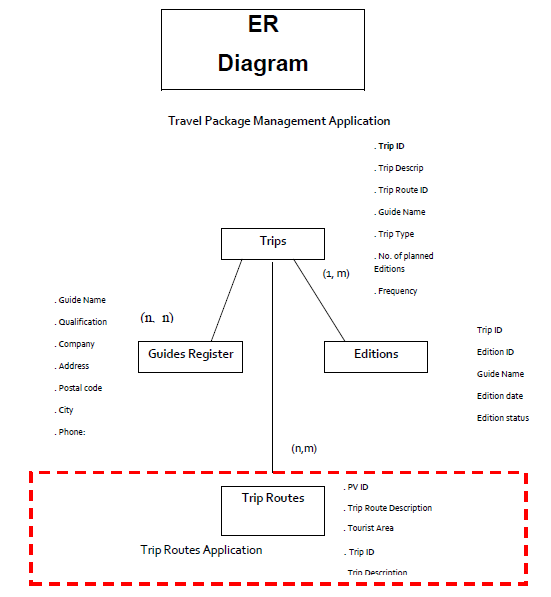
\includegraphics[width=10cm]{Sifp31.png}

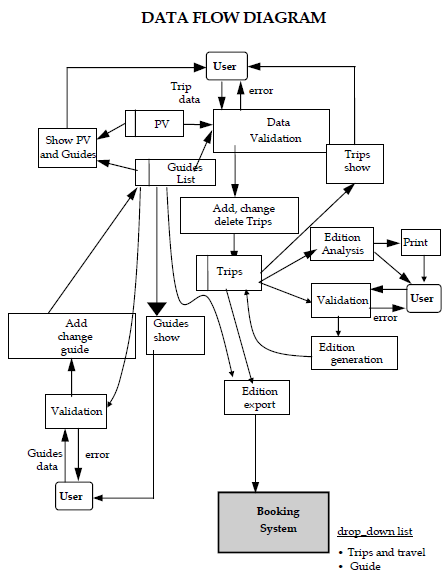
\includegraphics[width=10cm]{Sifp32.png}

\hypertarget{ux63a5ux4e58ux5ba2}{%
\subsubsection{答案与解读}\label{ux63a5ux4e58ux5ba2}}

共三个实体:\\

1.行程 (Trips)\\
2.导游登记册 (Guides Register)\\
3.行程路线(PV)\\

你可能会问:那些导游登记的各版本是否也应该是一个实体?(因需要花工夫开发)\\
这不应该是实体,原因:各版本必须依赖导游的信息挂在一起,不可以独立存在,就好比我们要维护导游的某版本信息,这个版本信息不能算另外一个实体,因为没有导游的话,版本信息是不能单独存在。\\


原则:不是根据是否要产生开发的工作量,而是从用户角度看,这实体能否独立存在和维护。否则功能点的估算就只是根据个人对开发工作量的估计,而不是从用户角度看功能的客观判断。(同样,行程里的版本也不能算是实体。)\\

行程管理,对用户来讲,都有新增、展示、修改、删除4个行为。在行程管理里,还有包括分析各版本,和管理行程版本等共4个行为。\\

导游管理,有新增、展示、修改 3个行为(没有删除)。\\

同步后台预订系统也是一行为,得出共 12(=4+4+3+1)行为,再加 3个实体。 计算简化功能点:每个实体 x7 ,每行为 x4.6 得出,共 76.2 (=3x7+12x4.6)简化功能点,详见下面列表: \\


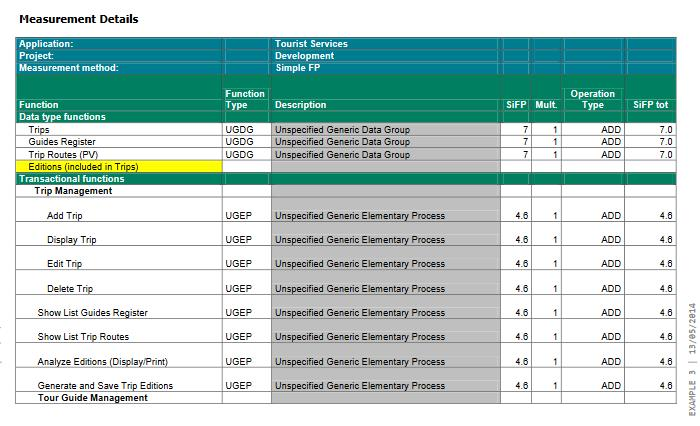
\includegraphics[width=10cm]{微信截图_20220325104633.jpg}


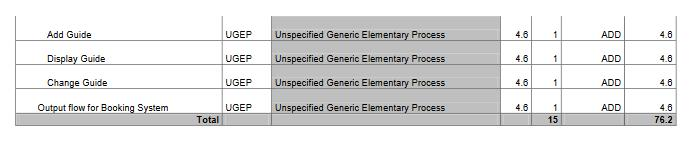
\includegraphics[width=10cm]{微信截图_20220325104709.jpg}


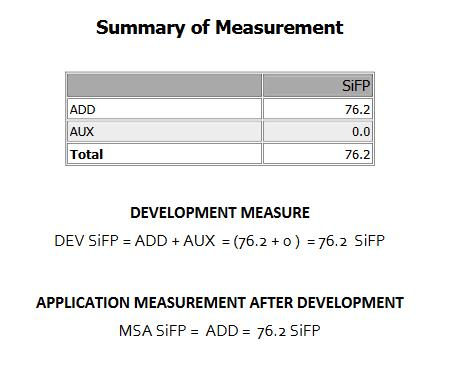
\includegraphics[width=10cm]{微信截图_20220325104725.jpg}

\hypertarget{ux4e0eux56fdux9645ux529fux80fdux70b9ifpugux7684ux504fux5dee}{%
\subsection{增强与维护(FEM)项目例子:旅游服务 Tourist Services}\label{ux4e0eux56fdux9645ux529fux80fdux70b9ifpugux7684ux504fux5dee}}

\hypertarget{ux63a5ux4e58ux5ba2}{%
\subsubsection{描述}\label{ux63a5ux4e58ux5ba2}}

基于以上旅游服务系统例子的需求为基础,客户提出以下软件功能增强与维护(FEM)\\

\hypertarget{ux63a5ux4e58ux5ba2}{%
\subsubsection{功能需求}\label{ux63a5ux4e58ux5ba2}}

\hypertarget{ux63a5ux4e58ux5ba2}{%
\subsubsection{RF01}\label{ux63a5ux4e58ux5ba2}}

功能增强维护后,行程(Trips)管理系统必须显示在PV文件中旅行国家的当前政治局势的信息。\\

\hypertarget{ux63a5ux4e58ux5ba2}{%
\subsubsection{RF02}\label{ux63a5ux4e58ux5ba2}}

有关导游经验的信息必须在导游登记档案的旅游领域(tourism)中处理。


\hypertarget{ux63a5ux4e58ux5ba2}{%
\subsubsection{RF03}\label{ux63a5ux4e58ux5ba2}}


必须提供用户那些最多被挑选的行程/旅行套餐的统计数据。

\hypertarget{ux63a5ux4e58ux5ba2}{%
\subsubsection{RF04}\label{ux63a5ux4e58ux5ba2}}

行程/旅游套餐必须送到相关政府部门备案。\\

\hypertarget{ux63a5ux4e58ux5ba2}{%
\subsubsection{答案与解读}\label{ux63a5ux4e58ux5ba2}}

新增两行为:统计,送政府部门备案\\
变更了4个行为:处理导游经验信息的增查改,和关于行程的变更(政治局势信息)\\
两实体,行程+导游,需有变更\\

动态功能点包括:\\
增加的功能点 9.2 (2 x 4.6),变更 32.4 (=4 x 4.6 + 2 x 7.0),没有删除,总共的动态简化功能点 41.6。\\

静态功能点依据上面例子的 76.2,加上FEM增加的功能点 9.2,得出变更后静态功能点 85.4。详见下面列表: \\



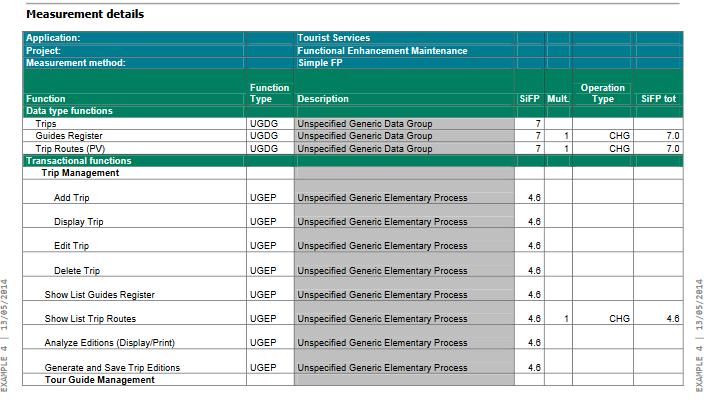
\includegraphics[width=10cm]{微信截图_20220325124602.jpg}


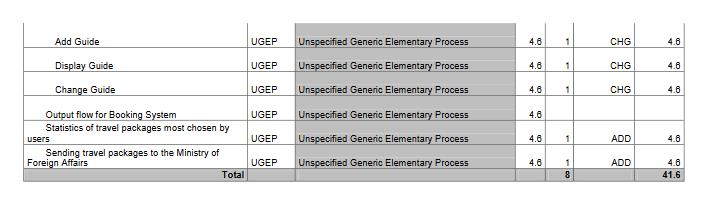
\includegraphics[width=10cm]{微信截图_20220325124630.jpg}

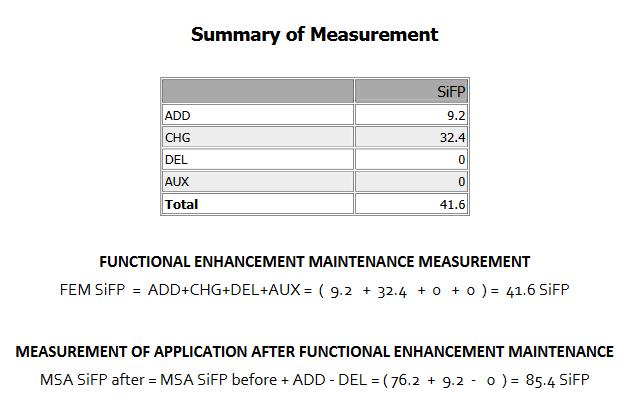
\includegraphics[width=10cm]{微信截图_20220325124706.jpg}






\hypertarget{ux4e0eux56fdux9645ux529fux80fdux70b9ifpugux7684ux504fux5dee}{%
\subsection{与国际功能点(IFPUG)的偏差}\label{ux4e0eux56fdux9645ux529fux80fdux70b9ifpugux7684ux504fux5dee}}

例子:

\begin{itemize}
\tightlist
\item
  新开发某会计付款系统
\item
  实体: 包括管理 发票 ,付款,供货商。
\item
  行为:包括对每个实体的展示,增加,修改,和删除/取消
\item
  使用IFPUG 数 EI, EO, EQ, ILF, EIF
  每类的调整前功能点数,加起来得出调整前功能点数FP=82
  (如想多了解IFPUG如何计算复杂度,参考附件)
\item
  使用SiFP 估算实体和行为数,计算得出 FP=104
\end{itemize}

%\href{文件:FPA_S11.jpg}{500px}

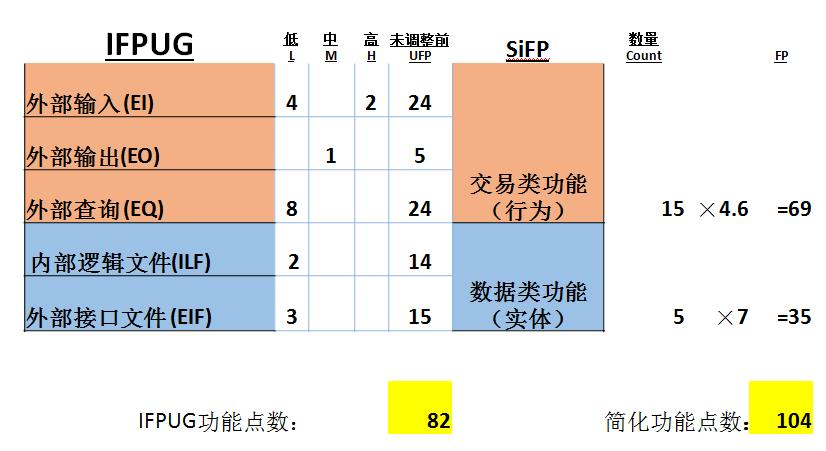
\includegraphics[width=10cm]{FPAS11.jpg}

\begin{itemize}
\tightlist
\item
  IFPUG / SiFP
  得出的实体数量,与行为数量都一样 (实体(=ILF+EIF)=5  行为
  (=EI+EO+EQ)=15)
\item
  因为简化功能点只是不区分实体与行为的复杂度(高中低),取平均值,原理一样,虽然个别估算有差异,但平均下来与IFPUG的估算没有结构性偏差
\end{itemize}

